\subsection{多边形的内角和}\label{subsec:czjh1-4-2}

我们知道,三角形的内角和等于 $180^\circ$, 怎样计算边数为 $n$ 的多边形的内角和呢?
如果能将多边形分成一些三角形,问题就解决了。

\begin{wrapfigure}[8]{r}{5cm}
    \centering
    \begin{tikzpicture}
    \tkzDefPoints{0/0/A_2, 1/-1/A_3, 3/-0.9/A_4, 4/0/A_5, 3.8/1/A_6, 2.5/1.6/A_n, 1/1.2/A_1, 1.8/0/O}

    \foreach \x in {1,...,5} {
        \pgfmathsetmacro{\n}{\x+1}
        \tkzDrawSegment(A_\x,A_\n)
        \tkzDrawSegment(A_\x,O)
    }
    \tkzDrawSegments(A_1,A_n  A_n,O  O,A_6)
    \tkzDrawSegment[dashed](A_6,A_n)

    \tkzLabelPoints[left](A_2)
    \tkzLabelPoints[below](A_3,A_4,O)
    \tkzLabelPoints[right](A_5,A_6)
    \tkzLabelPoints[above](A_n,A_1)
\end{tikzpicture}


    \caption{}\label{fig:czjh1-4-4}
\end{wrapfigure}

在已知 $n$ 边形 $A_1 A_2 A_3 \cdots A_n$ 内任取一点 $O$(图\ref{fig:czjh1-4-4}),
连结 $OA_1$、$OA_2$、$OA_3$、$\cdots$、$OA_n$,
这些线段将 $n$ 边形分成以 $O$ 为公共顶点的 $n$ 个三角形。
由此可得,$n$ 边形的内角和等于这 $n$ 个三角形的内角和
减去以 $O$ 为顶点的 $n$ 个角的和。
因为 $n$ 个三角形内角的和是 $n \cdot 180^\circ$,
以 $O$ 为顶点的 $n$ 个角的和是一个周角,等于 $360^\circ$,
所以 $n$ 边形的内角和是
$$ n \cdot 180^\circ - 360^\circ = (n - 2) \cdot 180^\circ \juhao $$

由此得到下面的定理:

\begin{dingli}[多边形内角和定理]
    $\bm{n}$ 边形的内角的和等于 $\bm{(n - 2) \cdot 180^\circ}$。
\end{dingli}

取多边形每一个内角的一个邻补角,它们相加的和叫做多边形的外角和。
因为多边形每一个内角与它的一个邻补角的和等于 $180^\circ$,
应用上面定理可以推算,$n$ 边形 $n$ 个外角的和等于
$$ n \cdot 180^\circ - (n - 2) \cdot 180^\circ = 360^\circ \juhao $$
于是得到:

\begin{tuilun}[推论1]
    任意多边形的外角和等于 $\bm{360^\circ}$。
\end{tuilun}

在第二章,我们学过两边分别平行的两个角的关系,现在,
我们应用多边形内角和定理来研究两边分别垂直的两个角的大小有什么关系。

\begin{wrapfigure}[8]{r}{5cm}
    \centering
    \begin{tikzpicture}
    \tkzDefPoints{0/0/A,  3/1/O}
    \tkzDefPoint(4,0){A_1}
    \tkzDefPoint(50:4){A_2}
    \tkzDefPointBy[projection= onto A--A_1](O)  \tkzGetPoint{B}
    \tkzDefPointBy[projection= onto A--A_2](O)  \tkzGetPoint{C}
    \tkzDefPointOnLine[pos=2.2](B,O)  \tkzGetPoint{E}
    \tkzDefPointOnLine[pos=1.5](C,O)  \tkzGetPoint{D}
    \tkzDrawSegments(A,A_1  A,A_2  B,E  C,D)
    \tkzMarkRightAngle(A,B,E)
    \tkzMarkRightAngle(A,C,D)
    \extkzLabelAngel[0.3](C,O,B){$1$}
    \extkzLabelAngel[0.5](B,O,D){$2$}
    \extkzLabelAngel[0.3](D,O,E){$3$}
    \extkzLabelAngel[0.5](E,O,C){$4$}
    \tkzLabelPoints[below](A,B)
    \tkzLabelPoints[right](D,E)
    \tkzLabelPoints[above left](C)
\end{tikzpicture}


    \caption{}\label{fig:czjh1-4-5}
\end{wrapfigure}

如图 \ref{fig:czjh1-4-5}, $\angle 1$ 的两边分别垂直于 $\angle A$ 的两边,那么,
因为 $\angle 1$ 和 $\angle A$ 是一个四边形的两个内角,
而这个四边形的另外两个内角都等于 $90^\circ$, 所以

$\angle 1 + \angle A = (4 - 2) \cdot 180^\circ - 2 \times 90^\circ = 180^\circ$,
即 $\angle 1$ 与 $\angle A$ 互补。

又 $\angle 2$、$\angle 3$、 $\angle 4$ 的两边也分别垂直于 $\angle A$ 的两边。

因为 $\angle 3 = \angle 1$, 所以 $\angle 3$ 和 $\angle A$ 也互补。

又因为 $\angle 2$ 和 $\angle A$ 都是 $\angle 1$ 的补角, 所以 $\angle 2 = \angle A$。

同理 $\angle 4 = \angle A$。 由此得到:

\begin{tuilun}[推论2]
    如果一个角的两边分别垂直于另一个角的两边,那么这两个角相等或互补。
\end{tuilun}

当两个角都是锐角或都是钝角时,这两个相等;
当两个角中一个是锐角一个是钝角时,这两个角互补。


\liti 已知一个多边形,它的内角和等于外角和的两倍,求这个多边形的边数。

\jie 设多边形的边数为 $n$, 因为它的内角和等于 $(n - 2) \cdot 180^\circ$,
外角和等于 $360^\circ$, 所以,
$$ (n - 2) \cdot 180^\circ = 2 \cdot 360^\circ \juhao $$

解得:\quad $n = 6$。

答:这个多边形的边数是 $6$。


\begin{figure}[htbp]
    \centering
    \begin{minipage}[b]{7cm}
        \centering
        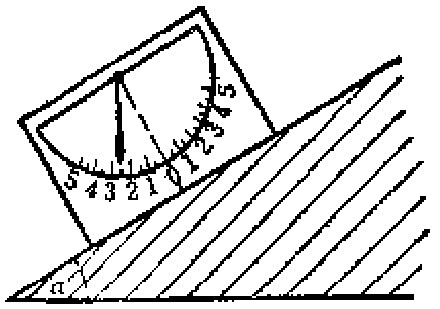
\includegraphics[width=5cm]{../pic/czjh1-ch4-06.png}
        \caption{}\label{fig:czjh1-4-6}
    \end{minipage}
    \qquad
    \begin{minipage}[b]{7cm}
        \centering
        \begin{tikzpicture}
    \tkzDefPoints{0/0/A, 4/0/B, 1/3/D}
    \tkzDefPoint(35:4){C}
    \tkzDefPointBy[projection= onto A--C](D)  \tkzGetPoint{O}
    \tkzDefPointBy[projection= onto A--B](D)  \tkzGetPoint{E}
    \tkzInterLL(A,C)(D,E)  \tkzGetPoint{M}
    \tkzDrawSegments(A,B  A,C  D,O)
    \tkzDrawSegment[->,>=Latex,thick](D,M)
    \tkzDrawSegment[dashed](M,E)
    \tkzMarkRightAngle[size=0.2](C,O,D)
    \tkzMarkRightAngle[size=0.2](B,E,D)
    \extkzLabelAngel[0.3](B,A,C){$\alpha$}
    \tkzLabelPoints[left](A)
    \tkzLabelPoints[below](E,B)
    \tkzLabelPoints[above](D)
    \tkzLabelPoints[right](C)
    \tkzLabelPoints[below](O)
\end{tikzpicture}


        \caption{}\label{fig:czjh1-4-7}
    \end{minipage}
\end{figure}


\liti 测斜坡的倾斜角可以用坡度板。坡度板上有半圆形的角度刻度,
$0^\circ$ 线垂直于板边, 在圆心处挂一自然下垂的金属指针, 把板边放在斜坡上,
看指针所指的度数, 就是斜坡的倾斜角 $\alpha$ 的度数。 说明它的道理。

\jie 按题意,画出坡度板测斜坡倾斜角的几何图形,如图 \ref{fig:czjh1-4-7}。

$\because$ \quad $DO \perp AC$, $DE \perp AB$,

且 \quad $\angle D < 90^\circ$, $\alpha < 90^\circ$,

$\therefore$ \quad $\angle \alpha = \angle D$ (两边分别垂直的两个锐角相等)。

所以,指针所指的度数就是斜坡的倾斜角 $\alpha$ 的度数。



\begin{lianxi}

\xiaoti{几边形的内角和等于它的外角和?}

\xiaoti{一个多边形的每一个外角都是 $72^\circ$, 这个多边形的内角和是多少度?}

\xiaoti{已知两组对应边互相垂直的两个角之差为 $35^\circ$, 求这两个角的度数。}

\end{lianxi}


